\documentclass[twoside]{book}

% Packages required by doxygen
\usepackage{calc}
\usepackage{doxygen}
\usepackage{graphicx}
\usepackage[utf8]{inputenc}
\usepackage{makeidx}
\usepackage{multicol}
\usepackage{multirow}
\usepackage{textcomp}
\usepackage[table]{xcolor}

% Font selection
\usepackage[T1]{fontenc}
\usepackage{mathptmx}
\usepackage[scaled=.90]{helvet}
\usepackage{courier}
\usepackage{amssymb}
\usepackage{sectsty}
\renewcommand{\familydefault}{\sfdefault}
\allsectionsfont{%
  \fontseries{bc}\selectfont%
  \color{darkgray}%
}
\renewcommand{\DoxyLabelFont}{%
  \fontseries{bc}\selectfont%
  \color{darkgray}%
}

% Page & text layout
\usepackage{geometry}
\geometry{%
  a4paper,%
  top=2.5cm,%
  bottom=2.5cm,%
  left=2.5cm,%
  right=2.5cm%
}
\tolerance=750
\hfuzz=15pt
\hbadness=750
\setlength{\emergencystretch}{15pt}
\setlength{\parindent}{0cm}
\setlength{\parskip}{0.2cm}
\makeatletter
\renewcommand{\paragraph}{%
  \@startsection{paragraph}{4}{0ex}{-1.0ex}{1.0ex}{%
    \normalfont\normalsize\bfseries\SS@parafont%
  }%
}
\renewcommand{\subparagraph}{%
  \@startsection{subparagraph}{5}{0ex}{-1.0ex}{1.0ex}{%
    \normalfont\normalsize\bfseries\SS@subparafont%
  }%
}
\makeatother

% Headers & footers
\usepackage{fancyhdr}
\pagestyle{fancyplain}
\fancyhead[LE]{\fancyplain{}{\bfseries\thepage}}
\fancyhead[CE]{\fancyplain{}{}}
\fancyhead[RE]{\fancyplain{}{\bfseries\leftmark}}
\fancyhead[LO]{\fancyplain{}{\bfseries\rightmark}}
\fancyhead[CO]{\fancyplain{}{}}
\fancyhead[RO]{\fancyplain{}{\bfseries\thepage}}
\fancyfoot[LE]{\fancyplain{}{}}
\fancyfoot[CE]{\fancyplain{}{}}
\fancyfoot[RE]{\fancyplain{}{\bfseries\scriptsize Generated on Tue Dec 24 2013 22:45:27 for ACSIGroupe35Curling by Doxygen }}
\fancyfoot[LO]{\fancyplain{}{\bfseries\scriptsize Generated on Tue Dec 24 2013 22:45:27 for ACSIGroupe35Curling by Doxygen }}
\fancyfoot[CO]{\fancyplain{}{}}
\fancyfoot[RO]{\fancyplain{}{}}
\renewcommand{\footrulewidth}{0.4pt}
\renewcommand{\chaptermark}[1]{%
  \markboth{#1}{}%
}
\renewcommand{\sectionmark}[1]{%
  \markright{\thesection\ #1}%
}

% Indices & bibliography
\usepackage{natbib}
\usepackage[titles]{tocloft}
\setcounter{tocdepth}{3}
\setcounter{secnumdepth}{5}
\makeindex

% Hyperlinks (required, but should be loaded last)
\usepackage{ifpdf}
\ifpdf
  \usepackage[pdftex,pagebackref=true]{hyperref}
\else
  \usepackage[ps2pdf,pagebackref=true]{hyperref}
\fi
\hypersetup{%
  colorlinks=true,%
  linkcolor=blue,%
  citecolor=blue,%
  unicode%
}

% Custom commands
\newcommand{\clearemptydoublepage}{%
  \newpage{\pagestyle{empty}\cleardoublepage}%
}


%===== C O N T E N T S =====

\begin{document}

% Titlepage & ToC
\hypersetup{pageanchor=false}
\pagenumbering{roman}
\begin{titlepage}
\vspace*{7cm}
\begin{center}%
{\Large A\-C\-S\-I\-Groupe35\-Curling }\\
\vspace*{1cm}
{\large Generated by Doxygen 1.8.4}\\
\vspace*{0.5cm}
{\small Tue Dec 24 2013 22:45:27}\\
\end{center}
\end{titlepage}
\clearemptydoublepage
\tableofcontents
\clearemptydoublepage
\pagenumbering{arabic}
\hypersetup{pageanchor=true}

%--- Begin generated contents ---
\chapter{Hierarchical Index}
\section{Class Hierarchy}
This inheritance list is sorted roughly, but not completely, alphabetically\-:\begin{DoxyCompactList}
\item \contentsline{section}{listeur\-Fic}{\pageref{classlisteur_fic}}{}
\item \contentsline{section}{parseur\-Fic}{\pageref{classparseur_fic}}{}
\item Q\-Main\-Window\begin{DoxyCompactList}
\item \contentsline{section}{Vue}{\pageref{class_vue}}{}
\end{DoxyCompactList}
\item \contentsline{section}{url\-Validator}{\pageref{classurl_validator}}{}
\end{DoxyCompactList}

\chapter{Class Index}
\section{Class List}
Here are the classes, structs, unions and interfaces with brief descriptions\-:\begin{DoxyCompactList}
\item\contentsline{section}{\hyperlink{classcontrol_vue}{control\-Vue} \\*Classe représentant le controleur principal }{\pageref{classcontrol_vue}}{}
\item\contentsline{section}{\hyperlink{classlisteur_fic}{listeur\-Fic} \\*Classe \hyperlink{classlisteur_fic}{listeur\-Fic} }{\pageref{classlisteur_fic}}{}
\item\contentsline{section}{\hyperlink{classparseur_fic}{parseur\-Fic} \\*Classe représentant le parseur de fichier }{\pageref{classparseur_fic}}{}
\item\contentsline{section}{\hyperlink{classurl_validator}{url\-Validator} \\*Classe représentant le valideur de fichier d'U\-R\-L }{\pageref{classurl_validator}}{}
\item\contentsline{section}{\hyperlink{class_vue}{Vue} \\*Classe représentant la vue principale }{\pageref{class_vue}}{}
\end{DoxyCompactList}

\chapter{File Index}
\section{File List}
Here is a list of all documented files with brief descriptions\-:\begin{DoxyCompactList}
\item\contentsline{section}{/home/toast/\-A\-C\-S\-I\-Groupe3\-Curling/\-A\-C\-S\-I\-Groupe35\-Curling/trunk/src/\hyperlink{parseur_fic_8h}{parseur\-Fic.\-h} \\*Parseur de fichier }{\pageref{parseur_fic_8h}}{}
\end{DoxyCompactList}

\chapter{Class Documentation}
\hypertarget{classlisteur_fic}{\section{listeur\-Fic Class Reference}
\label{classlisteur_fic}\index{listeur\-Fic@{listeur\-Fic}}
}


{\ttfamily \#include $<$listeur\-Fic.\-h$>$}

\subsection*{Public Member Functions}
\begin{DoxyCompactItemize}
\item 
void \hyperlink{classlisteur_fic_a9a035fde2cef3b9d70fbabfd98923493}{lister} (std\-::string nom\-Dossier)
\begin{DoxyCompactList}\small\item\em liste les fichiers d'un dossier \end{DoxyCompactList}\item 
Q\-File\-Info\-List \hyperlink{classlisteur_fic_a319d2a5d9de00dc984907b9256a7552b}{get\-Liste} ()
\begin{DoxyCompactList}\small\item\em retourne la liste des fichiers listés \end{DoxyCompactList}\item 
Q\-String\-List \hyperlink{classlisteur_fic_a769367aff699655d7e42450ac2f4a339}{get\-Q\-String\-Liste} ()
\begin{DoxyCompactList}\small\item\em retourne la liste des chemins des fichiers listés \end{DoxyCompactList}\item 
std\-::list$<$ std\-::string $>$ \hyperlink{classlisteur_fic_a859f53b053cd6f0d38bb36e6ae462b62}{get\-String\-Liste} ()
\begin{DoxyCompactList}\small\item\em retourne la liste des chemins des fichiers listés \end{DoxyCompactList}\end{DoxyCompactItemize}


\subsection{Detailed Description}
classe ... 

\subsection{Member Function Documentation}
\hypertarget{classlisteur_fic_a319d2a5d9de00dc984907b9256a7552b}{\index{listeur\-Fic@{listeur\-Fic}!get\-Liste@{get\-Liste}}
\index{get\-Liste@{get\-Liste}!listeurFic@{listeur\-Fic}}
\subsubsection[{get\-Liste}]{\setlength{\rightskip}{0pt plus 5cm}Q\-File\-Info\-List listeur\-Fic\-::get\-Liste (
\begin{DoxyParamCaption}
{}
\end{DoxyParamCaption}
)}}\label{classlisteur_fic_a319d2a5d9de00dc984907b9256a7552b}


retourne la liste des fichiers listés 

\begin{DoxyReturn}{Returns}
la liste des fichiers listés
\end{DoxyReturn}
Fonction qui retourne la liste des fichiers \hypertarget{classlisteur_fic_a769367aff699655d7e42450ac2f4a339}{\index{listeur\-Fic@{listeur\-Fic}!get\-Q\-String\-Liste@{get\-Q\-String\-Liste}}
\index{get\-Q\-String\-Liste@{get\-Q\-String\-Liste}!listeurFic@{listeur\-Fic}}
\subsubsection[{get\-Q\-String\-Liste}]{\setlength{\rightskip}{0pt plus 5cm}Q\-String\-List listeur\-Fic\-::get\-Q\-String\-Liste (
\begin{DoxyParamCaption}
{}
\end{DoxyParamCaption}
)}}\label{classlisteur_fic_a769367aff699655d7e42450ac2f4a339}


retourne la liste des chemins des fichiers listés 

\begin{DoxyReturn}{Returns}
le tableau des Q\-String/chemins des fichiers listés
\end{DoxyReturn}
Fonction qui retourne la liste des fichiers \hypertarget{classlisteur_fic_a859f53b053cd6f0d38bb36e6ae462b62}{\index{listeur\-Fic@{listeur\-Fic}!get\-String\-Liste@{get\-String\-Liste}}
\index{get\-String\-Liste@{get\-String\-Liste}!listeurFic@{listeur\-Fic}}
\subsubsection[{get\-String\-Liste}]{\setlength{\rightskip}{0pt plus 5cm}list$<$ string $>$ listeur\-Fic\-::get\-String\-Liste (
\begin{DoxyParamCaption}
{}
\end{DoxyParamCaption}
)}}\label{classlisteur_fic_a859f53b053cd6f0d38bb36e6ae462b62}


retourne la liste des chemins des fichiers listés 

\begin{DoxyReturn}{Returns}
le tableau de std\-::string/chemins des fichiers listés
\end{DoxyReturn}
Fonction qui retourne la liste des fichiers \hypertarget{classlisteur_fic_a9a035fde2cef3b9d70fbabfd98923493}{\index{listeur\-Fic@{listeur\-Fic}!lister@{lister}}
\index{lister@{lister}!listeurFic@{listeur\-Fic}}
\subsubsection[{lister}]{\setlength{\rightskip}{0pt plus 5cm}void listeur\-Fic\-::lister (
\begin{DoxyParamCaption}
\item[{std\-::string}]{nom\-Dossier}
\end{DoxyParamCaption}
)}}\label{classlisteur_fic_a9a035fde2cef3b9d70fbabfd98923493}


liste les fichiers d'un dossier 


\begin{DoxyParams}{Parameters}
{\em nom\-Dossier} & \-: le fichier a lire\\
\hline
\end{DoxyParams}
Méthode qui liste les fichiers dans un dossier dont le nom est donné en paramètre (nom\-Dossier) 

The documentation for this class was generated from the following files\-:\begin{DoxyCompactItemize}
\item 
/home/toast/\-A\-C\-S\-I\-Groupe3\-Curling/\-A\-C\-S\-I\-Groupe35\-Curling/src/\-Curling/\hyperlink{listeur_fic_8h}{listeur\-Fic.\-h}\item 
/home/toast/\-A\-C\-S\-I\-Groupe3\-Curling/\-A\-C\-S\-I\-Groupe35\-Curling/src/\-Curling/listeur\-Fic.\-cpp\end{DoxyCompactItemize}

\hypertarget{classparseur_fic}{\section{parseur\-Fic Class Reference}
\label{classparseur_fic}\index{parseur\-Fic@{parseur\-Fic}}
}


classe représentant le parseur de fichier  




{\ttfamily \#include $<$parseur\-Fic.\-h$>$}

\subsection*{Public Member Functions}
\begin{DoxyCompactItemize}
\item 
void \hyperlink{classparseur_fic_a450d9c873d69b8bd2dfbaf7f932d7f3d}{lire\-Fic} (std\-::string nom\-Fic)
\begin{DoxyCompactList}\small\item\em lis le fichier et y prend les url \end{DoxyCompactList}\item 
Q\-String\-List \hyperlink{classparseur_fic_aecce62c0c3fd85b703ba04bb955445fd}{get\-Urls} ()
\begin{DoxyCompactList}\small\item\em retourne les url lues \end{DoxyCompactList}\item 
void \hyperlink{classparseur_fic_ad2c99c1283f03ac105a2927aa9826021}{test\-Urls} ()
\begin{DoxyCompactList}\small\item\em test les url avec wget \end{DoxyCompactList}\end{DoxyCompactItemize}


\subsection{Detailed Description}
classe représentant le parseur de fichier 

classe gérant la lecture depuis un fichier à la recherche d'url 

\subsection{Member Function Documentation}
\hypertarget{classparseur_fic_aecce62c0c3fd85b703ba04bb955445fd}{\index{parseur\-Fic@{parseur\-Fic}!get\-Urls@{get\-Urls}}
\index{get\-Urls@{get\-Urls}!parseurFic@{parseur\-Fic}}
\subsubsection[{get\-Urls}]{\setlength{\rightskip}{0pt plus 5cm}Q\-String\-List parseur\-Fic\-::get\-Urls (
\begin{DoxyParamCaption}
{}
\end{DoxyParamCaption}
)}}\label{classparseur_fic_aecce62c0c3fd85b703ba04bb955445fd}


retourne les url lues 

\begin{DoxyReturn}{Returns}
le tableau d'url
\end{DoxyReturn}
Fonction qui retourne les url lues dans un fichier au préalable \hypertarget{classparseur_fic_a450d9c873d69b8bd2dfbaf7f932d7f3d}{\index{parseur\-Fic@{parseur\-Fic}!lire\-Fic@{lire\-Fic}}
\index{lire\-Fic@{lire\-Fic}!parseurFic@{parseur\-Fic}}
\subsubsection[{lire\-Fic}]{\setlength{\rightskip}{0pt plus 5cm}void parseur\-Fic\-::lire\-Fic (
\begin{DoxyParamCaption}
\item[{std\-::string}]{nom\-Fic}
\end{DoxyParamCaption}
)}}\label{classparseur_fic_a450d9c873d69b8bd2dfbaf7f932d7f3d}


lis le fichier et y prend les url 


\begin{DoxyParams}{Parameters}
{\em nom\-Fic} & \-: le fichier a lire\\
\hline
\end{DoxyParams}
Méthode qui lis le fichier passé en paramètre et accumule les url qu'il y trouve \hypertarget{classparseur_fic_ad2c99c1283f03ac105a2927aa9826021}{\index{parseur\-Fic@{parseur\-Fic}!test\-Urls@{test\-Urls}}
\index{test\-Urls@{test\-Urls}!parseurFic@{parseur\-Fic}}
\subsubsection[{test\-Urls}]{\setlength{\rightskip}{0pt plus 5cm}void parseur\-Fic\-::test\-Urls (
\begin{DoxyParamCaption}
{}
\end{DoxyParamCaption}
)}}\label{classparseur_fic_ad2c99c1283f03ac105a2927aa9826021}


test les url avec wget 

Fonction qui test les url lues 

The documentation for this class was generated from the following files\-:\begin{DoxyCompactItemize}
\item 
/home/toast/\-A\-C\-S\-I\-Groupe3\-Curling/\-A\-C\-S\-I\-Groupe35\-Curling/src/\-Curling/\hyperlink{parseur_fic_8h}{parseur\-Fic.\-h}\item 
/home/toast/\-A\-C\-S\-I\-Groupe3\-Curling/\-A\-C\-S\-I\-Groupe35\-Curling/src/\-Curling/parseur\-Fic.\-cpp\end{DoxyCompactItemize}

\hypertarget{classurl_validator}{\section{url\-Validator Class Reference}
\label{classurl_validator}\index{url\-Validator@{url\-Validator}}
}


classe représentant le valideur d(e fichier d'U\-R\-L  




{\ttfamily \#include $<$urlvalidator.\-h$>$}

\subsection*{Public Member Functions}
\begin{DoxyCompactItemize}
\item 
bool \hyperlink{classurl_validator_a337a9edaa44e76bda5a7ed3a345b0b78}{test\-Struct} (std\-::string p\-U\-R\-L)
\begin{DoxyCompactList}\small\item\em test si l'url est bien structurée \end{DoxyCompactList}\item 
bool \hyperlink{classurl_validator_a9993e82ddcaf00c655e3ad9221a10232}{test\-Vie} (std\-::string p\-U\-R\-L)
\begin{DoxyCompactList}\small\item\em retourne les url lues \end{DoxyCompactList}\end{DoxyCompactItemize}


\subsection{Detailed Description}
classe représentant le valideur d(e fichier d'U\-R\-L 

classe gérant les tests appliqués à une U\-R\-L 

\subsection{Member Function Documentation}
\hypertarget{classurl_validator_a337a9edaa44e76bda5a7ed3a345b0b78}{\index{url\-Validator@{url\-Validator}!test\-Struct@{test\-Struct}}
\index{test\-Struct@{test\-Struct}!urlValidator@{url\-Validator}}
\subsubsection[{test\-Struct}]{\setlength{\rightskip}{0pt plus 5cm}bool url\-Validator\-::test\-Struct (
\begin{DoxyParamCaption}
\item[{std\-::string}]{p\-U\-R\-L}
\end{DoxyParamCaption}
)}}\label{classurl_validator_a337a9edaa44e76bda5a7ed3a345b0b78}


test si l'url est bien structurée 


\begin{DoxyParams}{Parameters}
{\em p\-U\-R\-L} & \-: la chaine de caractere representant l'U\-R\-L \\
\hline
\end{DoxyParams}
\begin{DoxyReturn}{Returns}
booleen \-: Vrai si l'U\-R\-L est bien structurée, sinon Faux
\end{DoxyReturn}
Fonction qui test si l'U\-R\-L est bien construite et structurée grace à une expression régulière \hypertarget{classurl_validator_a9993e82ddcaf00c655e3ad9221a10232}{\index{url\-Validator@{url\-Validator}!test\-Vie@{test\-Vie}}
\index{test\-Vie@{test\-Vie}!urlValidator@{url\-Validator}}
\subsubsection[{test\-Vie}]{\setlength{\rightskip}{0pt plus 5cm}bool url\-Validator\-::test\-Vie (
\begin{DoxyParamCaption}
\item[{std\-::string}]{p\-U\-R\-L}
\end{DoxyParamCaption}
)}}\label{classurl_validator_a9993e82ddcaf00c655e3ad9221a10232}


retourne les url lues 


\begin{DoxyParams}{Parameters}
{\em p\-U\-R\-L} & \-: la chaine de caractere representant l'U\-R\-L \\
\hline
\end{DoxyParams}
\begin{DoxyReturn}{Returns}
le tableau d'url
\end{DoxyReturn}
Fonction qui test si l'U\-R\-L est bien vivante et accessible grace à une utilisation d'une commande utilisant \char`\"{}wget\char`\"{} (mode \char`\"{}-\/-\/spider\char`\"{}) 

The documentation for this class was generated from the following files\-:\begin{DoxyCompactItemize}
\item 
/home/toast/\-A\-C\-S\-I\-Groupe3\-Curling/\-A\-C\-S\-I\-Groupe35\-Curling/src/\-Curling/urlvalidator.\-h\item 
/home/toast/\-A\-C\-S\-I\-Groupe3\-Curling/\-A\-C\-S\-I\-Groupe35\-Curling/src/\-Curling/urlvalidator.\-cpp\end{DoxyCompactItemize}

\hypertarget{class_vue}{\section{Vue Class Reference}
\label{class_vue}\index{Vue@{Vue}}
}


classe représentant la vue principale  




{\ttfamily \#include $<$vue.\-h$>$}

Inheritance diagram for Vue\-:\begin{figure}[H]
\begin{center}
\leavevmode
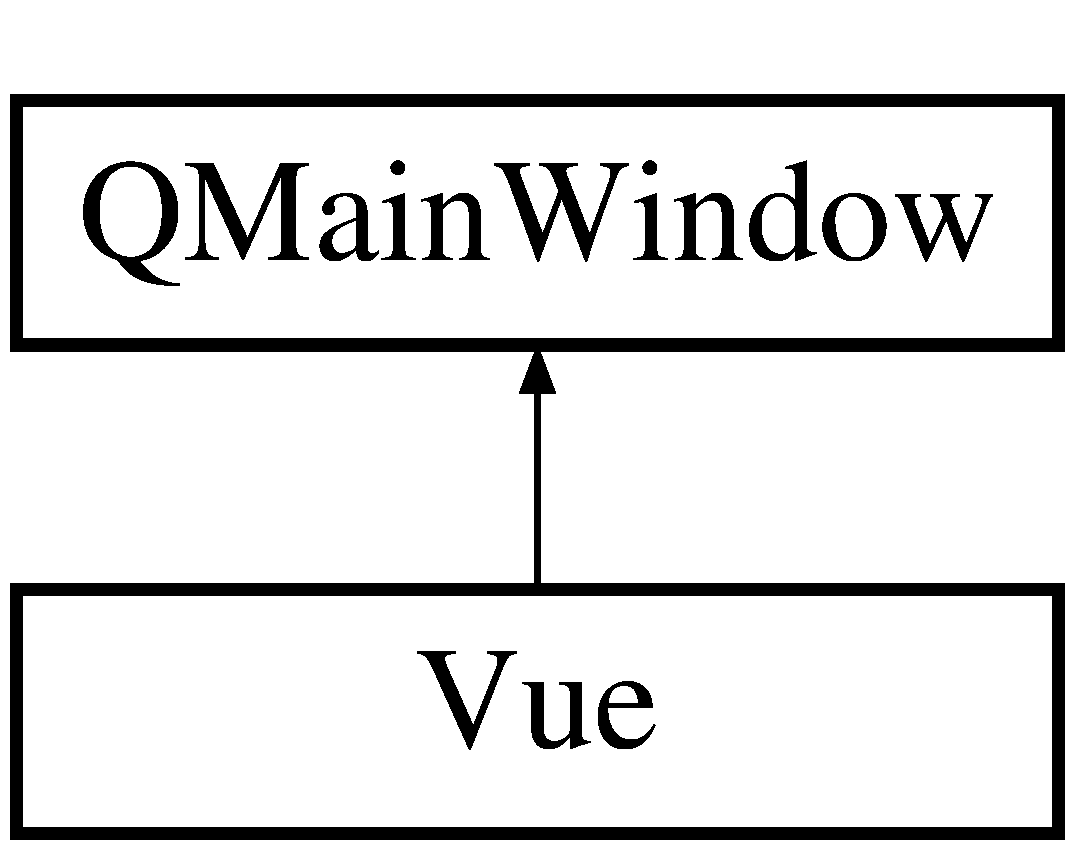
\includegraphics[height=2.000000cm]{class_vue}
\end{center}
\end{figure}
\subsection*{Public Slots}
\begin{DoxyCompactItemize}
\item 
void \hyperlink{class_vue_a70c0db80a2d27eb8097642b46e97f2d5}{clear\-Text} ()
\begin{DoxyCompactList}\small\item\em vide \char`\"{}zone\-Texte\char`\"{} \end{DoxyCompactList}\item 
void \hyperlink{class_vue_a71ae3f141fca897300185b8c2f9cc5c4}{add\-Ligne} (Q\-String ligne)
\begin{DoxyCompactList}\small\item\em ajoute une ligne a \char`\"{}zone\-Texte\char`\"{} \end{DoxyCompactList}\item 
void \hyperlink{class_vue_a8072d6b6002989f8d4c76d51b63468e0}{parcourir\-Appuyer} ()
\begin{DoxyCompactList}\small\item\em appelée sur pression de \char`\"{}parcourir\char`\"{} \end{DoxyCompactList}\item 
void \hyperlink{class_vue_ad3d78f8e2ad89c29c9a1e0c4588ae4ed}{parcourir\-Dossier\-Appuyer} ()
\begin{DoxyCompactList}\small\item\em appelée sur pression de \char`\"{}parcourir\-Dossier\char`\"{} \end{DoxyCompactList}\item 
void \hyperlink{class_vue_a7fb0d20950a6596a3eef78e244628682}{tester\-Appuyer} ()
\begin{DoxyCompactList}\small\item\em appelée sur pression de \char`\"{}tester\char`\"{} \end{DoxyCompactList}\end{DoxyCompactItemize}
\subsection*{Public Member Functions}
\begin{DoxyCompactItemize}
\item 
\hypertarget{class_vue_a10e5079d33b1916e6c38a698c92fa1e9}{{\bfseries Vue} (Q\-Widget $\ast$parent=0)}\label{class_vue_a10e5079d33b1916e6c38a698c92fa1e9}

\end{DoxyCompactItemize}


\subsection{Detailed Description}
classe représentant la vue principale 

classe gérant la vue principale 

\subsection{Member Function Documentation}
\hypertarget{class_vue_a71ae3f141fca897300185b8c2f9cc5c4}{\index{Vue@{Vue}!add\-Ligne@{add\-Ligne}}
\index{add\-Ligne@{add\-Ligne}!Vue@{Vue}}
\subsubsection[{add\-Ligne}]{\setlength{\rightskip}{0pt plus 5cm}void Vue\-::add\-Ligne (
\begin{DoxyParamCaption}
\item[{Q\-String}]{ligne}
\end{DoxyParamCaption}
)\hspace{0.3cm}{\ttfamily [slot]}}}\label{class_vue_a71ae3f141fca897300185b8c2f9cc5c4}


ajoute une ligne a \char`\"{}zone\-Texte\char`\"{} 


\begin{DoxyParams}{Parameters}
{\em ligne} & \-: le Q\-String a ajouter en fin de \char`\"{}zone\-Texte\char`\"{}\\
\hline
\end{DoxyParams}
Fonction qui ajoute une ligne (Q\-String) à la fin de \char`\"{}zone\-Texte\char`\"{} \hypertarget{class_vue_a70c0db80a2d27eb8097642b46e97f2d5}{\index{Vue@{Vue}!clear\-Text@{clear\-Text}}
\index{clear\-Text@{clear\-Text}!Vue@{Vue}}
\subsubsection[{clear\-Text}]{\setlength{\rightskip}{0pt plus 5cm}void Vue\-::clear\-Text (
\begin{DoxyParamCaption}
{}
\end{DoxyParamCaption}
)\hspace{0.3cm}{\ttfamily [slot]}}}\label{class_vue_a70c0db80a2d27eb8097642b46e97f2d5}


vide \char`\"{}zone\-Texte\char`\"{} 

Fonction qui vide \char`\"{}zone\-Texte\char`\"{} \hypertarget{class_vue_a8072d6b6002989f8d4c76d51b63468e0}{\index{Vue@{Vue}!parcourir\-Appuyer@{parcourir\-Appuyer}}
\index{parcourir\-Appuyer@{parcourir\-Appuyer}!Vue@{Vue}}
\subsubsection[{parcourir\-Appuyer}]{\setlength{\rightskip}{0pt plus 5cm}void Vue\-::parcourir\-Appuyer (
\begin{DoxyParamCaption}
{}
\end{DoxyParamCaption}
)\hspace{0.3cm}{\ttfamily [slot]}}}\label{class_vue_a8072d6b6002989f8d4c76d51b63468e0}


appelée sur pression de \char`\"{}parcourir\char`\"{} 

Fonction appelée lorsque le boutons \char`\"{}parcourir\char`\"{} est appuyé \hypertarget{class_vue_ad3d78f8e2ad89c29c9a1e0c4588ae4ed}{\index{Vue@{Vue}!parcourir\-Dossier\-Appuyer@{parcourir\-Dossier\-Appuyer}}
\index{parcourir\-Dossier\-Appuyer@{parcourir\-Dossier\-Appuyer}!Vue@{Vue}}
\subsubsection[{parcourir\-Dossier\-Appuyer}]{\setlength{\rightskip}{0pt plus 5cm}void Vue\-::parcourir\-Dossier\-Appuyer (
\begin{DoxyParamCaption}
{}
\end{DoxyParamCaption}
)\hspace{0.3cm}{\ttfamily [slot]}}}\label{class_vue_ad3d78f8e2ad89c29c9a1e0c4588ae4ed}


appelée sur pression de \char`\"{}parcourir\-Dossier\char`\"{} 

Fonction appelée lorsque le boutons \char`\"{}parcourir\-Dossier\char`\"{} est appuyé \hypertarget{class_vue_a7fb0d20950a6596a3eef78e244628682}{\index{Vue@{Vue}!tester\-Appuyer@{tester\-Appuyer}}
\index{tester\-Appuyer@{tester\-Appuyer}!Vue@{Vue}}
\subsubsection[{tester\-Appuyer}]{\setlength{\rightskip}{0pt plus 5cm}void Vue\-::tester\-Appuyer (
\begin{DoxyParamCaption}
{}
\end{DoxyParamCaption}
)\hspace{0.3cm}{\ttfamily [slot]}}}\label{class_vue_a7fb0d20950a6596a3eef78e244628682}


appelée sur pression de \char`\"{}tester\char`\"{} 

Fonction appelée lorsque le boutons \char`\"{}tester\char`\"{} est appuyé 

The documentation for this class was generated from the following files\-:\begin{DoxyCompactItemize}
\item 
/home/toast/\-A\-C\-S\-I\-Groupe3\-Curling/\-A\-C\-S\-I\-Groupe35\-Curling/src/\-Curling/\hyperlink{vue_8h}{vue.\-h}\item 
/home/toast/\-A\-C\-S\-I\-Groupe3\-Curling/\-A\-C\-S\-I\-Groupe35\-Curling/src/\-Curling/vue.\-cpp\end{DoxyCompactItemize}

\chapter{File Documentation}
\hypertarget{listeur_fic_8h}{\section{/home/toast/\-A\-C\-S\-I\-Groupe3\-Curling/\-A\-C\-S\-I\-Groupe35\-Curling/src/\-Curling/listeur\-Fic.h File Reference}
\label{listeur_fic_8h}\index{/home/toast/\-A\-C\-S\-I\-Groupe3\-Curling/\-A\-C\-S\-I\-Groupe35\-Curling/src/\-Curling/listeur\-Fic.\-h@{/home/toast/\-A\-C\-S\-I\-Groupe3\-Curling/\-A\-C\-S\-I\-Groupe35\-Curling/src/\-Curling/listeur\-Fic.\-h}}
}


listeur de fichier  


{\ttfamily \#include $<$iostream$>$}\\*
{\ttfamily \#include $<$fstream$>$}\\*
{\ttfamily \#include $<$string$>$}\\*
{\ttfamily \#include $<$Qt\-Core$>$}\\*
{\ttfamily \#include $<$Qt\-Gui/\-Qt\-Gui$>$}\\*
\subsection*{Classes}
\begin{DoxyCompactItemize}
\item 
class \hyperlink{classlisteur_fic}{listeur\-Fic}
\begin{DoxyCompactList}\small\item\em classe \hyperlink{classlisteur_fic}{listeur\-Fic} \end{DoxyCompactList}\end{DoxyCompactItemize}


\subsection{Detailed Description}
listeur de fichier \begin{DoxyAuthor}{Author}
E.\-Tosi 
\end{DoxyAuthor}
\begin{DoxyDate}{Date}
20.\-12.\-2013
\end{DoxyDate}
classe gérant les fichiers 
\hypertarget{parseur_fic_8h}{\section{/home/toast/\-A\-C\-S\-I\-Groupe3\-Curling/\-A\-C\-S\-I\-Groupe35\-Curling/src/\-Curling/parseur\-Fic.h File Reference}
\label{parseur_fic_8h}\index{/home/toast/\-A\-C\-S\-I\-Groupe3\-Curling/\-A\-C\-S\-I\-Groupe35\-Curling/src/\-Curling/parseur\-Fic.\-h@{/home/toast/\-A\-C\-S\-I\-Groupe3\-Curling/\-A\-C\-S\-I\-Groupe35\-Curling/src/\-Curling/parseur\-Fic.\-h}}
}


Parseur de fichier.  


{\ttfamily \#include $<$iostream$>$}\\*
{\ttfamily \#include $<$fstream$>$}\\*
{\ttfamily \#include $<$string$>$}\\*
{\ttfamily \#include $<$Qt\-Core$>$}\\*
{\ttfamily \#include \char`\"{}urlvalidator.\-h\char`\"{}}\\*
\subsection*{Classes}
\begin{DoxyCompactItemize}
\item 
class \hyperlink{classparseur_fic}{parseur\-Fic}
\begin{DoxyCompactList}\small\item\em classe représentant le parseur de fichier \end{DoxyCompactList}\end{DoxyCompactItemize}


\subsection{Detailed Description}
Parseur de fichier. \begin{DoxyAuthor}{Author}
E.\-Tosi 
\end{DoxyAuthor}
\begin{DoxyDate}{Date}
11.\-12.\-2013
\end{DoxyDate}
classe gérant la lecture depuis un fichier à la recherche d'url 
%--- End generated contents ---

% Index
\newpage
\phantomsection
\addcontentsline{toc}{part}{Index}
\printindex

\end{document}
